\section{Experimental Evaluation}

We have implemented \compiler\ in OCaml and it is currently able to produce C++
code that may be compiled directly or embedded in another application. We now
experimentally evaluate the query executors produced by \compiler\ in a mix of
application scenarios. These include the order book application described in the
introduction, which to the best of our knowledge cannot be supported by existing
stream processing engines, nor do they execute efficiently on traditional
databases, as well as a subset of the Linear Road stream processing benchmark
that simulates a toll-charging system on a highway, and lastly an end-to-end
warehouse loading and analysis based on generating a star schema from a TPC-H
dataset and computing aggregations on the star schema.

\subsection{Experimental Setup}
We experimentally evaluated \compiler\ on Dual Intel Xeon 5335 processor (8
cores, 2.0Ghz), 16Gb RAM, running Red Hat Enterprise Linux 4 (Linux Kernel
2.6.18). Note that \compiler\ does not yet produce query executors capable of
exploiting multicore processing, thus our results represent query performance on
a single core. Following the generation of C++ code, we used \texttt{g++} v4.3.2,
compiling with optimization level '-O3', and additional optimization parameters
for aggressive inlining and loop optimizations. We compare \compiler\ to two
other systems PostgreSQL v8.3.7, as well as a naive plan-based variant of
\compiler\ that simply produces C++ code directly from a query plan (instead of
rewriting to a tuple function).

\textbf{Data and query workloads.}
We discussed automated trading based on order book data in the introduction, and
use the VWAP query as one workload. The dataset feeding this query is the
TotalView-ITCH~\cite{totalview-url} historical order book from the NASDAQ stock
exchange for a 3-month period from December 2008 to February 2009, for the MSFT
(Microsoft) symbol. This application captures the need for standing queries on
temporal snapshots which may be arbitrarily modified with inserts, deletes and
updates, and where the application is self-governing in ensuring order books do
not grow unboundedly.

The second workload we consider is a stream processing workload, namely a subset
of the Linear Road benchmark~\cite{arasu-vldb:04} responsible for detecting
accidents and assessing tolls on the highway, which can be represented as pure
stream queries and do not need to access historical data. We are currently
implementing the full benchmark as part of ongoing work, and are expecting
further result improvements based on \compiler's ability to directly maintain
aggregated historical data as a standard data structure in the same process space
as the query executor, unlike other streaming engines which either rely on
embedded databases such BerkeleyDB (Aurora/Borealis), or have no support for
querying historical data (STREAM).

The third workload is an example of our warehouse loading application, where we
use \compiler\ to jointly process a data integration query loading a warehouse
from OLTP databases, and an aggregation query on the warehouse. We emulate the
data integration step by using a data cleaning and transformation query to
convert a TPC-H dataset into a star schema, as described in the Star Schema
Benchmark (SSB)~\cite{poneil-ssb:07}. We then evaluate query 4.1 from SSB on the
transformed TPC-H dataset. Note this all occurs in one single query compiled down
with \compiler.




\subsection{\compiler\ Performance}

\begin{figure}
\begin{center}
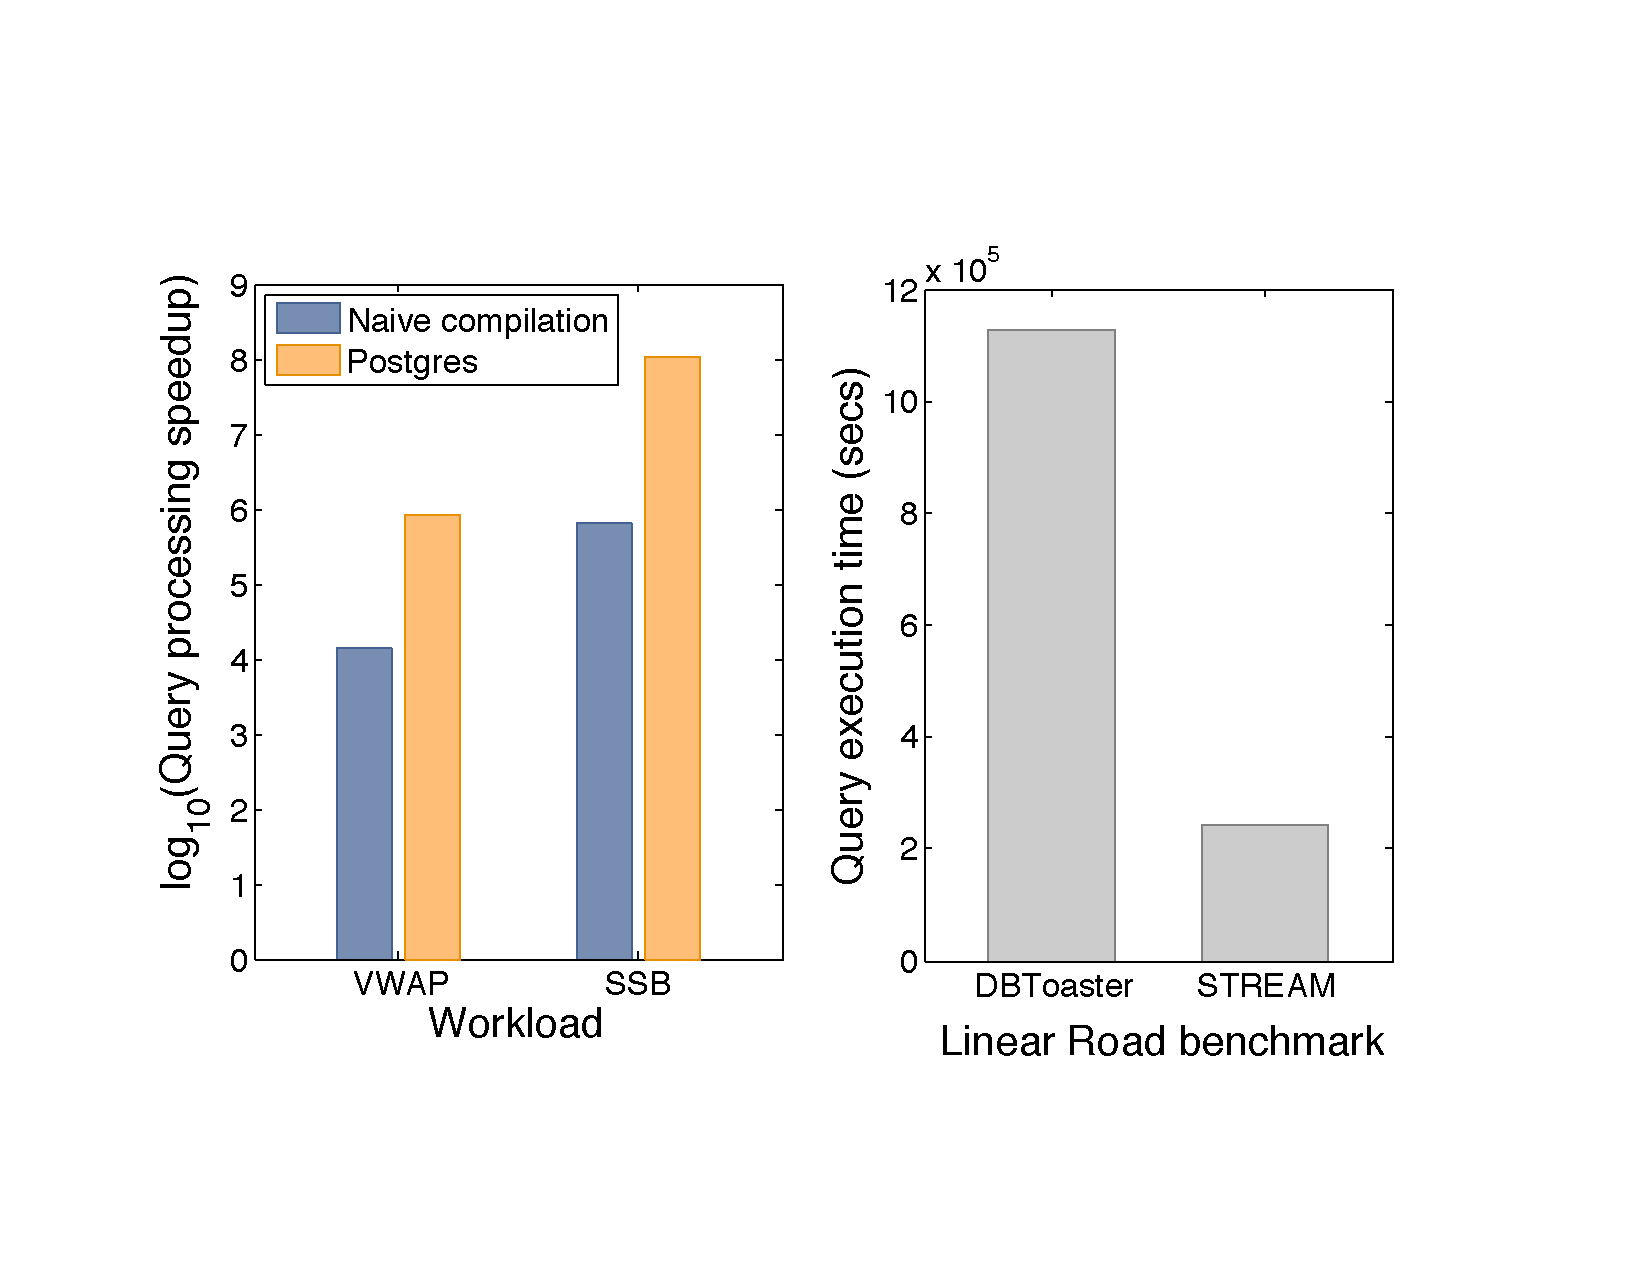
\includegraphics[scale=0.25]{../plots/toaster_comparison}
\end{center}
\caption{Query processing performance comparison of compiled query executors
generated by DBToaster and plan compilation, Postgres and STREAM}
\label{fig:dbtperf}
\end{figure}

\textbf{Query Processing.}
Figure~\ref{fig:dbtperf} illustrates the query processing performance of
\compiler\ compared to plan-based compilation and PostgreSQL for the VWAP and SSB
workloads, and to the Stanford STREAM engine for Linear Road. First we describe
the execution models of the VWAP and SSB queries on our three comparison points.
We use both plan-based compilation and PostgreSQL to query temporal snapshots by
repetitively querying changing base relations, and consider the average
processing time across these repetitions. In contrast, \compiler\ performs
per-tuple processing, producing a query result after each tuple, much like online
aggregation. Note that the query results are equivalent on those snapshots for
which all three systems produce results.

Figure~\ref{fig:dbtperf}i. displays the query processing speedup per result
refresh by \compiler, that is it compares this average processing time from
plan-based compilation and PostgreSQL, to the per-tuple processing cost of
\compiler. This metric captures a ratio of the overhead involved in producing a
new result. We do not consider stream processing engines in the VWAP or SSB
scenario, since they cannot capture the arbitrary order of inserts, deletes and
updates present in these workloads.
Figure~\ref{fig:dbtperf}ii illustrates the tuple throughput of \compiler\ and
STREAM on the Linear Road benchmark. Here we implemented all window functionality
with temporal range predicates, and \compiler\ used a doubly linked list-based
implementation of windows as described in the previous section. This figure shows
that even in pure stream processing scenarios, \compiler\ is able to outperform a
stream processing engine by a factor of 5x, outlining the benefits of creating
compiled query executors. As we described above, we expect this gap to widen as
we address more complex stream queries involving processing patterns and
aggregated historical data.

\textbf{Query refresh limits.}

\begin{figure}
\begin{center}
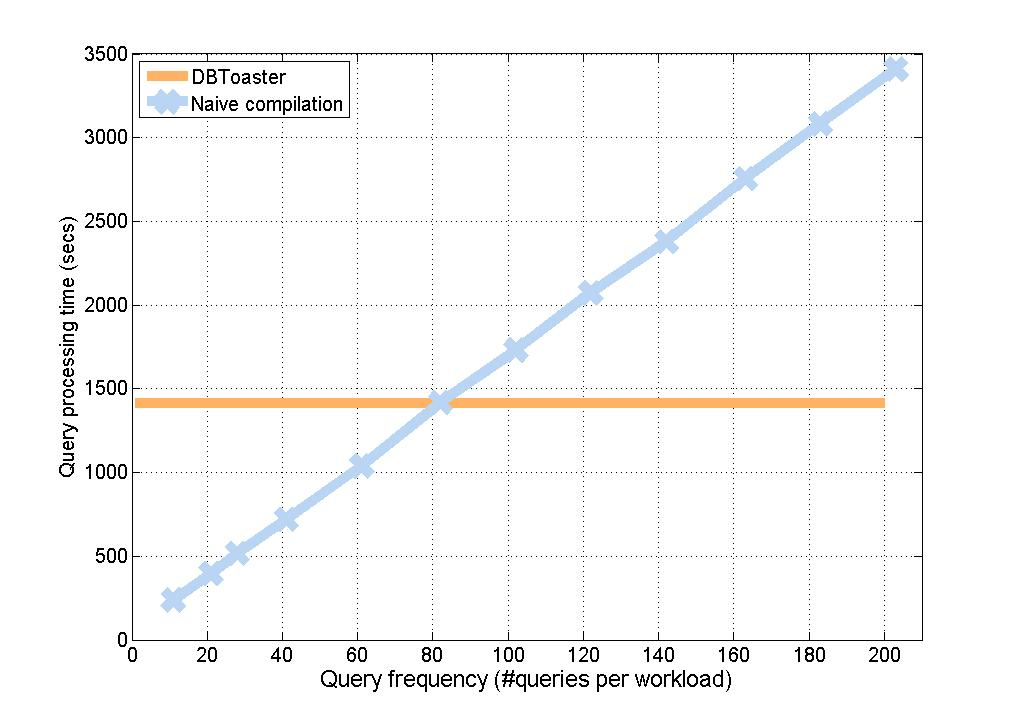
\includegraphics[scale=0.25]{../plots/vwap_query_freq_dn}
\end{center}
\caption{Query frequency limit for VWAP application, indicating the
query execution frequency beyond which DBToaster outperforms the naive query
plan compilation technique.}
\label{fig:vwap_query_freq}
\end{figure}

\begin{figure}
\begin{center}
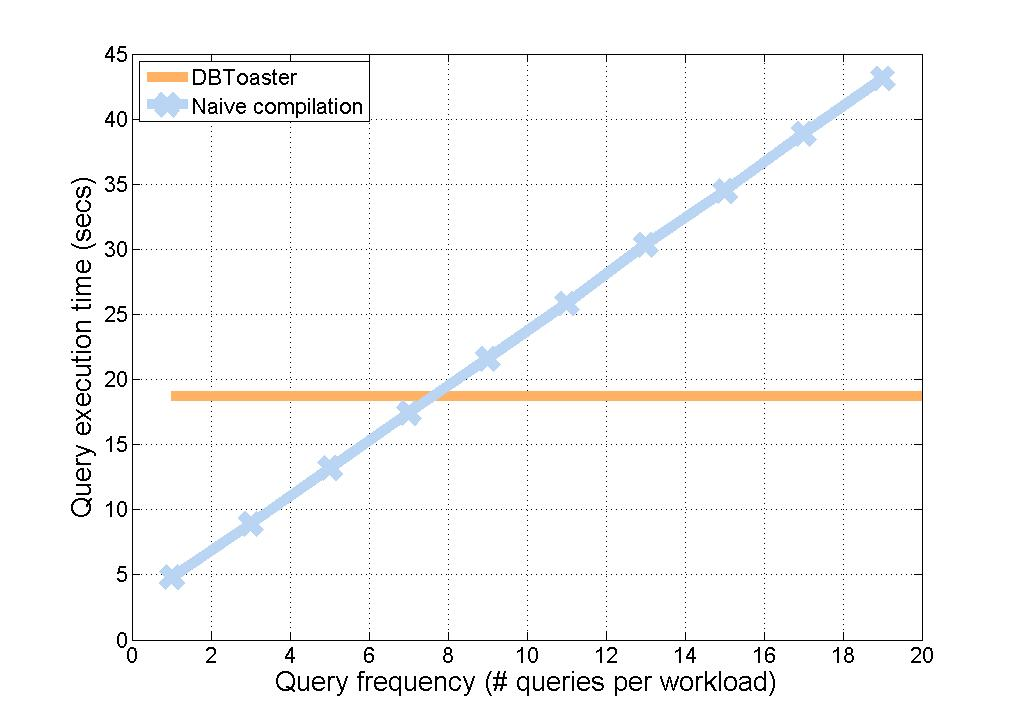
\includegraphics[scale=0.25]{../plots/ssb_query_freq_dn}
\end{center}
\caption{Query frequency limit for warehouse loading application, indicating the
query execution frequency beyond which DBToaster outperforms the naive query
plan compilation technique.}
\label{fig:ssb_query_freq}
\end{figure}

Figure~\ref{fig:vwap_query_freq} shows the threshold for repetitively executing
VWAP queries in both the plan-based compiled executor and PostgreSQL, before such
execution becomes more costly than simply processing the whole workload with
\compiler\ (hence the constant execution time for \compiler). This figure
essentially shows the cumulative execution cost of refreshing query results.
Clearly, for ad-hoc one-time queries, creating a compiled plan executor will
outperform incremental execution. As an aside, we believe \compiler\ will be
extremely useful to the database community at large even for this kind of usage,
since compilation overheads which are not shown here, remain low enough to
justify compiling prior to ad-hoc query execution. Returning to our VWAP
scenario, we see the threshold for using \compiler\ is at around 80 queries in
the 1-day order book workload. While this might seem a large number, automated
trading applications require the highest resolution view available on order books
and a limit of 80 queries would mean querying roughly once every 5 minutes, an
unacceptable query rate for trading firms.

Figure~\ref{fig:ssb_query_freq} shows the equivalent plot for the SSB workload.
Here the threshold is much smaller due to the increased query complexity of
having to join multiple large tables when executing a query. In this case, the
relative performance of \compiler\ improves against both alternative
implementations due to its ability to avoid fully producing intermediate join
results by using aggregate views and by using tuple functions to maintain these
views, enabling \compiler\ to attain a query repetition limit of approximately 8
plan-compiled queries.


\begin{figure}
\begin{center}
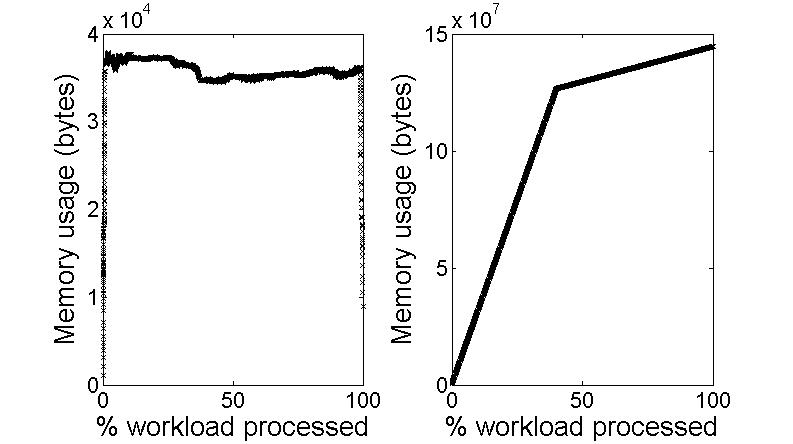
\includegraphics[scale=0.3]{../plots/mem_usage}
\end{center}
\caption{Memory usage of \compiler's map data structures in the i) VWAP and ii)
SSB workloads.}
\label{fig:memusage}
\end{figure}

\textbf{Memory consumption.}
We instrumented the code generated by \compiler\ to profile the memory used in
maintaining map data structures during tuple processing.
Figure~\ref{fig:memusage}i and ii shows memory consumption for the VWAP
and SSB workload respectively. These two workloads lie in highly different
application domains and as such exhibit different memory requirements.
Figure~\ref{fig:memusage}i confirms our expectation that order books do not
grow unbounded and that they do not require windowing semantics. In fact, with
a footprint of approximately 36Kb for a single stock's orderbook, \compiler\
could certainly be used to process the entire NASDAQ order book extremely
efficiently compared to existing systems on a single server.
In contrast the SSB workload displays a growing memory usage as we scan over the
lineitem, orders and customers tables, performing query execution. Note that the
kink in the plot arises when we switch from processing lineitem, the dominant
table in the workload, to the order and customers tables (whose tuples are
roughly the same size hence the equivalent gradient). By the end of processing
the query workload consumes approximately 150Mb. This is still smaller than the
input scale factor 1 TPC-H database used in this experiment, indicating we do
not keep the full input relations in main memory. Furthermore, although we
started execution from an empty database in this example, the low overhead
leaves plenty of room to maintain aggregate views from prior database loads,
making \compiler\ a viable high-performance framework for answering aggregate
queries.

We briefly comment that there are a couple of alternative implementations we
are currently in the process of evaluating as comparison points, namely
trigger-based implementations of incremental query processing, and incremental
view maintenance schemes. We are confident \compiler\ will exhibit significant
gains over both these techniques for the following reasons. First much of the
motivation behind stream processing engines lies in the fact that trigger
processing infrastructure in modern databases tend to be inefficient for
high volume update rates due to the implementation of cascades and the
concurrency model of triggers. This result was demonstrated by the Linear Road
benchmark. Second, incremental view maintenance algorithms are designed to
reuse the query processing infrastructure already present in relational
databases, hence they reuse the same interpreter as for mainline query
execution. We anticipate that our compiled executors will demonstrate
similar advantages over such interpreted evaluation.


\comment{
Dataset:

\begin{itemize}
  \item TotalView-ITCH dataset: 3 month's worth of MSFT order book messages
  taken from NASDAQ, (~2.2Gb dataset).
  \item Orderbook schema: day, time in us since beginning of day, order id,
  order type, share volume, bid/ask price
\end{itemize}

Queries:

\begin{verbatim}
select * from
  (select ax_bids.mmid, abs(
    sum(ax_bids.volume*
      (act_now.expected_price - ax_bids.price)) -
    sum(ax_asks.volume*
      (ax_asks.price - act_now.expected_price)))
    as ax_bias
  from
    (select mmid, price, volume from bids
       where mmid in axs) as ax_bids,
    (select mmid, price, volume from asks
       where mmid in axs) as ax_asks,
    (select expected_price
        from technical_indicator
        where entrance_condition)
    as act_now
  where ax_bids.mmid = ax_asks.mmid
  group by ax_bids.mmid) as sneaky_ax,
where ax_bias > 10000
\end{verbatim}

Figures:

\begin{enumerate}
  \item Takeaway experiment: end-to-end throughput comparison for a variety of
  insert/update/delete rates. Requires replay speed parameter in data loader.
  Comparison points include Postgres, naive compilation, simple version
  of \compiler, \compiler\ with lazy evaluation, \compiler\ with bulk insert
  mode at 2 or 3 different chunk sizes.

  \item Detail experiment: analyse effect of bulk loading operations compared to
  simple compiler, on a variety of queries, e.g. selectivities and keys.
  Dependent variables for plots: cache hit rates for locality analysis,
  throughput to understand pipelining effects. Is there anything lower lever we
  can do for pipelining?

  \item Detail experiment: selectivity experiment, comparing \compiler\ w/ lazy
  eval, and w/ bulk loading (separately) to next best, for a variety of
  join selectivities and keys.

  \item Detail experiment: space vs recomputation analysis, where we vary the
  maps we keep between extremes of maps from simple decomposition, to full base
  tables.

  \item Quality of compiled code, and compiler effect? e.g. speed provided with
  different -O flags?

\end{enumerate}
}